\documentclass{standalone}

\usepackage[OT1]{fontenc}
\renewcommand*\familydefault{\sfdefault}
\usepackage{helvet,sfmath}
\usepackage{siunitx}

\usepackage{tikz}
\usetikzlibrary{arrows,calc,patterns}
\usepackage{tikz,tkz-euclide}

\definecolor{BlueDefault}{rgb}{0.2,0.2,0.7}

\begin{document}

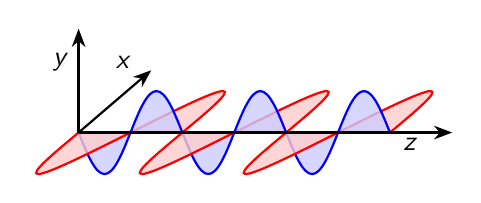
\begin{tikzpicture}[x=0.75pt,y=0.75pt,yscale=-1,xscale=1]
    %uncomment if require: \path (0,300); %set diagram left start at 0, and has height of 300
    
    %Shape: Wave 
    \draw[thick, blue, fill = blue!20, fill opacity=0.8]    (100,144) .. controls (104.08,154.25) and (107.98,164) .. (112.5,164) .. controls (117.02,164) and (120.92,154.25) .. (125,144);
    \draw[thick, red, fill = red!20, fill opacity=0.8]  (100,144) .. controls (87.69,154.25) and (76,164) .. (80.51,164) .. controls (85,164) and (104.54,154.25) .. (125,144);

    \draw[thick, red, fill = red!20, fill opacity=0.8]  (125,144) .. controls (145.47,133.75) and (164.98,124) .. (169.5,124) .. controls (174,124) and (162.32,133.75) .. (150,144);
    \draw[thick, blue, fill = blue!20, fill opacity=0.8]    (125,144) .. controls (129.08,133.75) and (132.98,124) .. (137.5,124) .. controls (142.02,124) and (145.92,133.75) .. (150,144);

    \draw[thick, blue, fill = blue!20, fill opacity=0.8]    (150,144) .. controls (154.08,154.25) and (157.98,164) .. (162.5,164) .. controls (167.02,164) and (170.92,154.25) .. (175,144);
    \draw[thick, red, fill = red!20, fill opacity=0.8]  (150,144) .. controls (137.69,154.25) and (125.99,164) .. (130.5,164) .. controls (135,164) and (154.54,154.25) .. (175,144);

    \draw[thick, red, fill = red!20, fill opacity=0.8]  (175,144) .. controls (195.47,133.75) and (214.98,124) .. (219.5,124) .. controls (224,124) and (212.32,133.75) .. (200,144);
    \draw[thick, blue, fill = blue!20, fill opacity=0.8]    (175,144) .. controls (179.08,133.75) and (182.98,124) .. (187.5,124) .. controls (192.02,124) and (195.92,133.75) .. (200,144);

    \draw[thick, blue, fill = blue!20, fill opacity=0.8]    (200,144) .. controls (204.08,154.25) and (207.98,164) .. (212.5,164) .. controls (217.02,164) and (220.92,154.25) .. (225,144);
    \draw[thick, red, fill = red!20, fill opacity=0.8]  (200,144) .. controls (187.69,154.25) and (175.99,164) .. (180.5,164) .. controls (185,164) and (204.54,154.25) .. (225,144);

    \draw[thick, red, fill = red!20, fill opacity=0.8] (225,144).. controls (245.47,133.75) and (264.98,124) .. (269.5,124) .. controls (274,124) and (262.34,133.74) .. (250,144);
    \draw[thick, blue, fill = blue!20, fill opacity=0.8]    (225,144) .. controls (229.08,133.75) and (232.98,124) .. (237.5,124) .. controls (242.02,124) and (245.92,133.75) .. (250,144) ;

    %Coordinate
    \draw[thick, -Stealth] (100,144) to (280,144);
    \draw[thick, -Stealth] (100,144) to (100,94);
    \draw[thick, -Stealth] (100,144) to (135,114);
    \draw 
    (130,110) node[left]{\(x\)}
    (100,110) node[left]{\(y\)}
    (260,142) node[below]{\(z\)}
    ;
    \end{tikzpicture}

\end{document}